% =====================================================================
%  3.1 Data cleaning and preprocessing
% =====================================================================
\subsection{Data Cleaning and Preprocessing}
\label{sec:preprocessing}

The test year 2018 is cut from the raw files before any processing, so not even a
forward-fill can carry test information into development. \Cref{tab:cleaning} lists each step and
the reason for it.

\begin{table}[H]
  \centering
  \small
  \caption{Cleaning steps. Counts refer to 2015--2017.}
  \label{tab:cleaning}
  \begin{tabularx}{\linewidth}{@{}p{2.6cm} Y Y@{}}
    \toprule
    Step & What we do & Why \\
    \midrule
    Time zone & Parse the \code{+01:00/+02:00} offsets as UTC (Coordinated Universal Time), convert to Europe/Madrid.
      & Demand follows the local clock; in UTC the morning peak would shift by one hour between
        winter and summer. \\
    Day $\times$ 24 grid & Spring-forward days get an empty 02:00 slot (not scored); the duplicated
      02:00 of autumn days is averaged.
      & Lags are looked up as ``same local hour, $k$ days ago''. A shift of 168 rows would be one
        hour off for a week after each clock change. \\
    Weather duplicates & Drop 3{,}076 duplicated (city, hour) rows; all duplicates carry identical
      temperatures (asserted in code).
      & Otherwise the merge multiplies rows. \\
    City names & Strip \code{" Barcelona"}. & A leading space creates a sixth ``city''. \\
    Units & Kelvin $\rightarrow$ $^\circ$C. & Readable degree-day bases. \\
    One-hour spikes & Set a load value to missing when it deviates by more than 15\% from the mean
      of its two neighbours while the neighbours agree within 10\%.
      & A national drop of 12\,GW (gigawatts) that recovers within one hour is a recording error. Thresholds of
        15, 20 and 25\% flag the same hours (3 in 2015--2017, 1 in 2018). \\
    Missing target & 34 raw missing hours plus the flagged spikes are never trained on or scored.
      & We do not score against invented values. \\
    Missing lag input & Forward-fill at most 3 hours.
      & Uses the past only; interpolation would use future values. \\
    Real outliers & Kept (midnight drops, holidays).
      & They are real events; the TSO forecast drops at the same hours. \\
    Weather aggregation & Simple mean of the five cities.
      & No external data needed and both models see the same variable. No population weights
        (limitation). \\
    \bottomrule
  \end{tabularx}
\end{table}

\paragraph{Time alignment.}
If timestamps mark the start of each hour, solar generation should peak around 13:00--14:00 local
time and temperature in mid-afternoon. \Cref{fig:alignment} confirms this: solar peaks at hour 13
and temperature at 16:00. Load and weather share the same time axis, so no shift is needed. Our
information cutoff (data up to hour 08 of $D-1$ for a 10:00 issue) is safe under either timestamp
convention.

\begin{figure}[H]
  \centering
  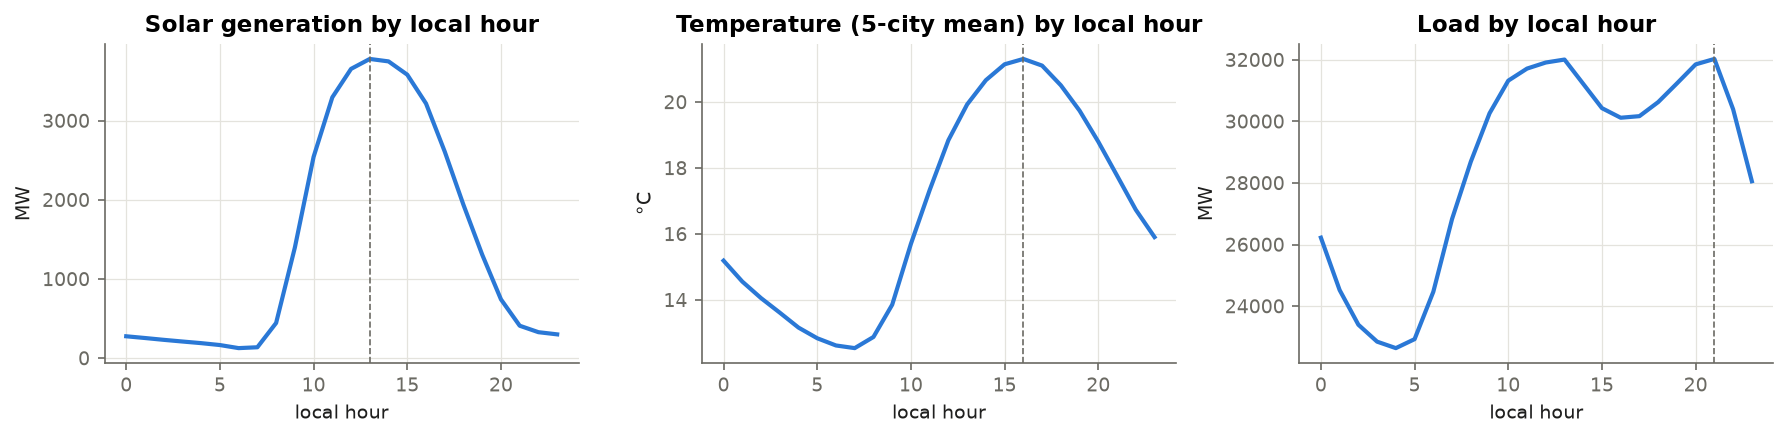
\includegraphics[width=\linewidth]{01_alignment_by_hour.png}
  \caption{Mean solar generation, temperature and load by local hour (2015--2017). Dashed lines mark
           the peak hour.}
  \label{fig:alignment}
\end{figure}
